% Options for packages loaded elsewhere
\PassOptionsToPackage{unicode}{hyperref}
\PassOptionsToPackage{hyphens}{url}
%
\documentclass[
  12pt,
]{article}
\usepackage{amsmath,amssymb}
\usepackage{iftex}
\ifPDFTeX
  \usepackage[T1]{fontenc}
  \usepackage[utf8]{inputenc}
  \usepackage{textcomp} % provide euro and other symbols
\else % if luatex or xetex
  \usepackage{unicode-math} % this also loads fontspec
  \defaultfontfeatures{Scale=MatchLowercase}
  \defaultfontfeatures[\rmfamily]{Ligatures=TeX,Scale=1}
\fi
\usepackage{lmodern}
\ifPDFTeX\else
  % xetex/luatex font selection
\fi
% Use upquote if available, for straight quotes in verbatim environments
\IfFileExists{upquote.sty}{\usepackage{upquote}}{}
\IfFileExists{microtype.sty}{% use microtype if available
  \usepackage[]{microtype}
  \UseMicrotypeSet[protrusion]{basicmath} % disable protrusion for tt fonts
}{}
\makeatletter
\@ifundefined{KOMAClassName}{% if non-KOMA class
  \IfFileExists{parskip.sty}{%
    \usepackage{parskip}
  }{% else
    \setlength{\parindent}{0pt}
    \setlength{\parskip}{6pt plus 2pt minus 1pt}}
}{% if KOMA class
  \KOMAoptions{parskip=half}}
\makeatother
\usepackage{xcolor}
\usepackage[margin=1in]{geometry}
\usepackage{graphicx}
\makeatletter
\def\maxwidth{\ifdim\Gin@nat@width>\linewidth\linewidth\else\Gin@nat@width\fi}
\def\maxheight{\ifdim\Gin@nat@height>\textheight\textheight\else\Gin@nat@height\fi}
\makeatother
% Scale images if necessary, so that they will not overflow the page
% margins by default, and it is still possible to overwrite the defaults
% using explicit options in \includegraphics[width, height, ...]{}
\setkeys{Gin}{width=\maxwidth,height=\maxheight,keepaspectratio}
% Set default figure placement to htbp
\makeatletter
\def\fps@figure{htbp}
\makeatother
\setlength{\emergencystretch}{3em} % prevent overfull lines
\providecommand{\tightlist}{%
  \setlength{\itemsep}{0pt}\setlength{\parskip}{0pt}}
\setcounter{secnumdepth}{5}
\usepackage{setspace} \usepackage{amsmath} \usepackage{graphicx} \usepackage{array} \usepackage{caption} \usepackage{longtable} \usepackage{booktabs} \usepackage{multirow} \usepackage{enumitem} \renewcommand{\arraystretch}{1} \captionsetup[table]{skip=5pt} \setstretch{1.5}
\ifLuaTeX
  \usepackage{selnolig}  % disable illegal ligatures
\fi
\usepackage[]{natbib}
\bibliographystyle{apalike}
\IfFileExists{bookmark.sty}{\usepackage{bookmark}}{\usepackage{hyperref}}
\IfFileExists{xurl.sty}{\usepackage{xurl}}{} % add URL line breaks if available
\urlstyle{same}
\hypersetup{
  pdftitle={Supplementary Material for Annual Review 22/23},
  pdfauthor={Zijian Zark Wang},
  hidelinks,
  pdfcreator={LaTeX via pandoc}}

\title{Supplementary Material for Annual Review 22/23}
\author{Zijian Zark Wang}
\date{August 14, 2023}

\begin{document}
\maketitle

\hypertarget{introduction}{%
\section{Introduction}\label{introduction}}

In this document, I present three pieces of work.

The first is a novel model of intertemporal choice, which I term as
``attentional discounted utility'' (ADU). The model incorporates
attentional mechanism into the expected discounted utility framework. It
assumes that people have limited attention to allocate across sequential
outcomes, and tend to pay more attention to the outcomes with larger
rewards. The model is consistent with a known empirical phenomenon in
intertemporal choice termed the ``hidden zero effect''. I focus on a
certain variant of ADU, that is, ADU with the Shannon cost function
(ADUS), and show how this can explain a broad set of decision anomalies.

The model was presented in the most recent annual review, and since
then, has undergone further clarification and refinement. Specifically,
I outline the following behavioral implications of ADUS: (1) the
requirement for the magnitude effect on curvature of utility function
can be relaxed; (2) it specifies a novel condition for the common
difference effect; (3) the discount function can perform an inverse-S
shape, which is consistent with some evidence; (4) it offers an
alternative account for S-shaped value function; (5) whether decision
makers are attentive or inattentive to decision task influences the
consistency of their choices. Moreover, I present an axiomatic
characterization of ADUS.

The second is an experimental test on whether (and how) attentional
mechanism can influence intertemporal choice. It is a new section, added
after the most recent annual review. I conducted two pilot studies and
am working on pre-registration at the moment of submitting this
document. The purpose of this experiment is to examine the key
assumptions in my model. In this experiment, participants are required
to choose between different sequences of rewards. I make two predictions
for the experimental results. First, extending the sequence length will
dilute the attention resources available for each specific period (given
people have limited attention to allocate across the periods), which
will make people less sensitive to changes in the amount of reward
offered in each period. Second, increasing reward amount in one period
will shift attention from other periods to this particular period; thus,
people will be less sensitive to changes in reward amount in the other
periods. Similar behavioral patterns were observed in a pilot study.

The third is an experiment aiming to test how people jointly evaluate
risky outcomes and efforts. This experimental design originates from an
idea I proposed two years ago. Findings from this experiment may help
clarify some issues in rational inattention theories. I am working on
the experimental program.

These three pieces of work may correspond to three chapters of my
thesis. Each piece of work is presented in Section \ref{2}, Section
\ref{3}, and Section \ref{4} respectively. During the upcoming two
months, I hope to complete the main analyses in the first piece of work.
The experiment in the second piece of work will be implemented in one
month; then, I plan to run a follow-up test in the subsequent two
months. The experiment in the third piece of work may be implemented by
the end of this year. Hopefully, I will be working on additional
analyses early next year, then complete the thesis in July, 2024. A full
schedule of work is presented at the end of the document.

\hypertarget{attentional-discounted-utility}{%
\section{\texorpdfstring{Attentional Discounted Utility
\label{2}}{Attentional Discounted Utility }}\label{attentional-discounted-utility}}

\hypertarget{the-model}{%
\subsection{The Model}\label{the-model}}

Expected discounted utility framework has been widely used in behavioral
and economic research. Given a sequence of rewards
\(X_T=[x_0,x_1,...,x_T]\), which yields reward \(x_t\) in time period
\(t\),\footnote{I use uppercase letters to represent a sequence and
  lowercase letters to represent each element within the sequence.}
\(t \in \{0,1,...,T\}\), the expected discounted utility of \(X_T\) can
be calculated by\[
EDU(X_T)= \mathbb{E}\left[\sum_{t=0}^T d_t u(x_t)\right]
\]where \(d_t\) is the discounting factor of time period \(t\), reward
level \(x_t\) is a random variable defined on \(\mathbb{R}_{\geq 0}\),
\(u(.)\) denotes the decision maker's instantaneous utility function,
\(u'>0\), \(u''<0\). The time length of this sequence, denoted by \(T\),
is finite.

The aim of this section is to incorporate attentional mechanism into
this valuation process of reward sequences. I assume that a decision
maker allocates attention across sequential outcomes when processing
information about rewards, and attends more to the outcomes with larger
rewards. I define the models that contain such features as
\emph{Attentional Discounted Utility} (ADU) models. Specifically, I
focus on a particular form of ADU, which I term as \emph{ADU with the
Shannon cost function} (ADUS). ADUS retains the architecture of expected
discounted utility, but simply modifies the conventional discounting
factor \(d_t\) to \(w_t\), which I refer to as an attention weight
hereafter, where \(w_t\) is calculated by

\begin{equation}\tag{1}\label{eq:wt}
w_t = \frac{d_t e^{\frac{u(x_t)}{\lambda}}}{\sum_{\tau=0}^T d_\tau e^{\frac{u(x_\tau)}{\lambda}}}
\end{equation}

In Equation (\ref{eq:wt}), \(w_t\) adopts a form resembling a logistic
function. It indicates three properties of attention. First, the sum of
all \(w_t\) equals 1. Under this constraint, an increase in attention
weight assigned to one period will result in a reduction in that for
some other periods, which indicates a shift of attention. Second,
\(w_t\) is increasing in \(x_t\), indicating the decision maker is
inclined to allocate more attention to periods with larger potential
rewards. This is in line with existing evidence, suggesting people often
pay more attention to pleasant information and less to unpleasant
information.\footnote{Many studies have suggested information has
  hedonic value. \citet{golman_information_2017} provides a good review
  for the relevant literature. The tendency to avoid paying attention to
  unpleasant information is sometimes called ostrich effect.
  \citet{galai_ostrich_2006}, \citet{sicherman_financial_2016} and
  \citet{quispe-torreblanca_attention_2022} find the evidence of ostrich
  effect in financial markets. Moreover, \citet{olafsson_ostrich_2017}
  find people are more likely to log in their bank accounts when they
  have more cash holdings and less debt in the accounts.} Third, \(w_t\)
is anchored in \(d_t\). This indicates that the conventional discounting
factor \(d_t\) can represent the initial attention weight assigned to
each period, and the psychological process of attention adjustment
(converting \(d_t\) to \(w_t\)) is costly. The parameter \(\lambda\)
quantifies the cost of attention adjustment. Notably, \(w_t\) is
positive for every period \(t\) within the sequence.

I provide two rationales for Equation (\ref{eq:wt}). The first is based
on rational inattention theories. The second is an axiomatic theory. I
present the first here and discuss the second in Section \ref{axiom}.

The rational inattention theories investigate how the cost or capacity
of acquiring information may impact relevant decision-making processes.
In ADU, it is assumed that when evaluating a reward sequence, the
decision makers tends to pay more attention to information with a higher
hedonic value, and the information that she could receive a
substantially large reward at some time is perceived as more
(hedoically) valuable than the information that she could receive only a
small reward at the same time. Consequently, as more information about
the sequence is acquired, her allocation of attention weights may
deviate more from its initial allocation. Notably, this attention
adjustment process triggers a cognitive cost. The decision maker needs
to balance the benefit of focusing on the information with higher value
and the cognitive cost of shifting attention. Her objective thus can be
viewed as to maximize an attention-weighted value of information at some
cost.

The necessary notations and definitions are described as follows. Let
\(S_T=[s_0,s_1,...,s_T]\) be a potential realization of \(X_T\), and
\(\mathcal{S}(X_T)\) be the support of \(X_T\), i.e.~the smallest set
containing any potentially realized sequence \(S_T\), where
\(\mathcal{S}(X_T)\subseteq \mathbb{R}_{\geq 0}^{T+1}\). Let \(w(s_t)\)
denote the attention weight assigned to outcome \(s_t\), and
\(\mathcal{W}\) denote the matrix consisting of all \(w(s_t)\), i.e.~the
attention weights for all periods in all potential realizations of
\(X_T\). For simplicity, I assume the value of each piece of information
is proportional to the instantaneous utility of a reward in each period.
Under this assumption, we can directly use the \emph{constrained optimal
discounting} problem\emph{,} termed by Noor and Takeoka
\citetext{\citeyear{noor_optimal_2022}; \citeyear{noor_constrained_2023}},
to define the process that generates \(\mathcal{W}\). The formal
definition is given by Definition 1.

\textbf{Definition 1}: Let \(W\) be the set containing all possible
realizations of \(\mathcal{W}\). Given a stochastic reward sequence
\(X_T\), the following optimization problem is called the
\emph{constrained optimal discounting} problem for \(X_T\):\[ 
\begin{aligned}
\max_{\mathcal{W}\in W}  \quad & \sum_{S_T\in \mathcal{S}(X_T)}\sum_{t=0}^T w(s_t)u(s_t) - C(\mathcal{W}) \\
s.t. \quad &  \sum_{S_T\in \mathcal{S}}\sum_{t=0}^T w(s_t)=m \\
& w(s_t)> 0 \text{ for all } S_T \text{ and } t\in\{0,1,…,T\} \\
\end{aligned}
\]where \(m\) is a constant,
\(C:[0,m]^{T+1}\rightarrow \mathbb{R}_{>0}\) is called \emph{information
cost} function, \(\partial C/\partial w(s_t)>0\) and
\(\partial^2 C/\partial w(s_t)^2>0\). That is, the information cost is
increasing and convex in \(w(s_t)\).

The process in Definition 1 determines the attention weight assigned to
each potential outcome in each time period. After that, the decision
maker' objective becomes to choose the option with the highest ADU,
where ADU is calculated by
\(\sum_{S_T\in\mathcal{S}}\sum_{t=0}^T w(s_t) u(s_t)\).

A well-known specification of \(C(.)\) is the Shannon cost function,
proposed by \citet{matejka_rational_2015}. The Shannon cost function was
originally used to justify the multinominal logit model in discrete
choice analysis, and so far has been widely discussed in rational
inattention literature. To construct this style of information cost
function, \citet{matejka_rational_2015} introduce three assumptions. The
first is that the sum of all weights is 1, i.e.~\(m\equiv1\). The second
is, before acquiring any information, the decision maker establishes an
initial weight allocation for different attributes (time periods), which
remains invariant across states. The weights are then updated in a
manner consistent with Bayes' rule. In ADU setting, it means
\(d_t=\sum_{S_T\in \mathcal{S}(X_T)} w(s_t)\). The third assumption is,
the information cost is linear to the information gains, measured by
Shannon mutual information. That
is,\[ C(w)= \lambda \sum_{S_T\in \mathcal{S}(X_T)}\sum_{t=0}^T w(s_t) \log\left(\frac{w(s_t)}{d_t p(S_T)}\right) \]where
\(\lambda\) is a parameter denoting unit cost of information
(\(\lambda>0\)), \(p(S_T)\) is the probability that \(S_T\) occurs. With
the Shannon cost function, the constrained optimal discounting problem
can be easily solved by Lagrangian method, and the solution is the same
as Equation (\ref{eq:wt}). \footnote{In each certain state \(S_T\),
  \(w_t\) in Equation (\ref{eq:wt}) can be defined by
  \(w_t\equiv w(s_t)/p(S_T)\).}

\hypertarget{related-literature}{%
\subsection{Related Literature}\label{related-literature}}

The present model is related to two kinds of models - endogenous time
preference and rational inattention. In a seminal paper about endogenous
time preference, \citet{becker_endogenous_1997} assume the decision
maker can increase the discounting factor for a future period by
spending resources in imagining or focusing on it. Such resources enters
the budget constraint, hence reduces the total amount of rewards that
the decision maker can obtain. On the contrary, the present model does
not make any specific assumption about budget constraint. The cost that
the decision maker pays to adjust attention is totally cognitive, and
the attention weights are subject to only a cognitive constraint.

In rational inattention models, one typical setting involves a decision
maker paying cognitive cost to learn the values of various options, then
determining the optimal probability for selecting each option
\citep{caplin_rationally_2022, mackowiak_rational_2023}.
\citet{steiner_rational_2017} propose a dynamic choice model to account
for status quo bias and behavioral inertia based on this typical
setting. The present model extends this setting by adding assumptions to
how the decision maker will determine the optimal weight assigned to
each specific outcome realized at each time. These assumptions
contribute to the research in how the value of an option is calculated
based on the information acquired in mind.

Moreover, \citet{gabaix_myopia_2017} assume that, in intertemporal
choice, the true value of a reward in each period is unknown. The
decision maker observes some noisy signals of it and estimates it using
Bayes' rule. The assumption is similar to the present model; yet, they
focus on how the decision maker infers the true value from the observed
signals, while the present model investigates how she integrates those
signals. \citet{gershman_rationally_2020} extend the thought of
\citet{gabaix_myopia_2017} and investigate how the decision maker
optimizes the precision of such signals under a certain information
constraint. The discounting factor derived from their model is also
increasing in reward magnitude, and it can be viewed as a special case
of the present model.

\hypertarget{behavioral-implications}{%
\subsection{Behavioral Implications}\label{behavioral-implications}}

\hypertarget{adu-is-generally-consistent-with-hidden-zero-effect}{%
\subsubsection{ADU is generally consistent with ``hidden zero
effect''}\label{adu-is-generally-consistent-with-hidden-zero-effect}}

Suppose a decision maker faces a choice between a small sooner reward
(SS) and a larger later reward (LL). The hidden zero effect
\citep{magen_hidden-zero_2008} implies she should exhibit more patience
if both SS and LL are framed as sequences rather than being framed as
single-period rewards. For instance, consider SS\textsubscript{0}:
``receive £100 today'', and LL\textsubscript{0}: ``receive £120 in 6
months''. Suppose we also have

\setlength{\leftskip}{1cm}

SS\textsubscript{1}: ``receive £100 today and £0 in 6 months''

LL\textsubscript{1}: ``receive £0 today and £120 in 6 months''

\setlength{\leftskip}{0pt}

The hidden zero effect suggests people are more likely to prefer
LL\textsubscript{1} over SS\textsubscript{1} than preferring
LL\textsubscript{0} over SS\textsubscript{0}. Subsequent research (e.g.
\citet{read_value_2017}) suggests the effect is asymmetric. That is,
shifting SS\textsubscript{0} to SS\textsubscript{1} and keeping
LL\textsubscript{0} unchanged do increase patience, whereas shifting
LL\textsubscript{0} to LL\textsubscript{1} and keeping
SS\textsubscript{0} unchanged cannot increase patience. This is
naturally compatible with attentional discounted utility.

To illustrate, imagine that the framing of sequence length can influence
how the decision maker may perceive it. For SS\textsubscript{0}, the
decision maker perceives the length of sequence as ``today''; for
SS\textsubscript{1}, she perceives the length as ``6 months''. According
to ADU, in the former case, she can allocate no attention to the future;
while in the latter case, she needs to pay some attention to future
periods, which contain no reward. Thus, the attention allocated to the
current period decreases when shifting from SS\textsubscript{0} to
SS\textsubscript{1} (given total capacity of attention is limited). This
leads to a decrease in the value of sequence. By contrast, shifting from
LL\textsubscript{0} to LL\textsubscript{1} does not change the length of
sequence, thus does not change the value.

One might wonder for a period with no reward, why the attention weight
may still be positive (``why should I pay attention to a period when
there is no reward present''). The hidden zero effect provides an
empirical reason. Additionally, from the theoretical view, attention
acts as a filter that determines which information could enter awareness
or working memory.\footnote{Such a view can be traced back to the
  bottleneck theories of attention, which starts from
  \citet{broadbent_perception_1958}.} If the decision maker is aware
about the information that the reward is zero in a certain period, it
implies attention may have already been directed to that period.

Hereafter, I focus on ADU with the Shannon cost function (ADUS) and
document five implications of the ADUS model in intertemporal choice.
Each of them can be mathematically proved.

\hypertarget{the-requirement-of-magnitude-effect-on-utility-function-can-be-relaxed-under-adus}{%
\subsubsection{The requirement of magnitude effect on utility function
can be relaxed under
ADUS}\label{the-requirement-of-magnitude-effect-on-utility-function-can-be-relaxed-under-adus}}

In conventional discounted utility models, to make the magnitude effect
holds true, the elasticity of utility function needs to be increasing
with reward level \citep{loewenstein_anomalies_1992}. This requirement
might be too strong so that many commonly used utility functions (such
as power and CARA utility functions) does not satisfy it. By contrast,
note in Equation (\ref{eq:wt}), \(w_t\) is increasing in \(x_t\). This
implies that when comparing SS and LL, the decision maker could exhibit
more patience toward larger reward levels, which relaxes the requirement
for the magnitude effect.

To illustrate how specifically ADUS relaxes this requirement, we should
derive how a delayed reward is valued in ADUS. Suppose the value of
``receive a certain reward \(x_T\) in period \(T\)'' is calculated by
\(w_T \cdot u(x_T)\). Then assuming the initial attention weight is in
exponential style, that is \(d_t\equiv\delta^t\) (\(0<\delta\leq1\)), we
should have

\begin{equation}\tag{2}\label{eq:w2}  
w_T = \frac{1}{1+G(T)e^{-u(x_T)/\lambda}}  
\end{equation}

and

\begin{equation}\tag{3}\label{eq:gt} 
G(T) = \left\{ 
\begin{aligned} 
& \frac{1}{1-\delta}(\delta^{-T}-1) \; ,& 0<\delta<1\\ 
& T\; ,& \delta=1
\end{aligned} \right. 
\end{equation}

It can be proved that, if Equation (\ref{eq:w2}) and (\ref{eq:gt}) are
both satisfied, for all \(x_T>0\), power utility function
\(u(x_T)={x_T}^\gamma\) with \(0<\gamma<1\), satisfies the curvature
requirement for magnitude effect, and when \(x_T\) is greater than a
positive finite number, CRRA utility function
\(u(x_T)=1-e^{-\gamma x_T}\) with \(\gamma>0\), also satisfies it.

\hypertarget{adus-specifies-a-novel-condition-for-common-difference-effect}{%
\subsubsection{ADUS specifies a novel condition for common difference
effect}\label{adus-specifies-a-novel-condition-for-common-difference-effect}}

According to the common difference effect
\citep{loewenstein_anomalies_1992}, suppose a decision maker is
indifferent between SS and LL, increasing the time delay before
receiving the reward in both options by a same amount can lead the
decision maker to prefer LL over SS.

The ADU models provide an alternative account for common difference
effect. Given attention is limited, when the delay of reward is
extended, that is, we insert some periods with zero reward into the
existing sequence, the newly inserted periods will grab attention from
other periods. As people tend to attend more to periods with larger
rewards, in LL, the period when a positive reward is delivered will
experience less attention being diverted compared to that in SS. This
disparity in attention weighing can lead to a preference for LL over SS.

Regarding the Shannon cost function, assuming initial time preference is
stationary, i.e.~\(d_t=\delta^t\), we can derive from Equation
(\ref{eq:w2}) and (\ref{eq:gt}) the conditions for common difference
effect. Clearly, if \(\delta=1\), the attention weight \(w_T\) will
follow a hyperbolic style. In this case, the common difference effect
will always hold true.

If \(0<\delta<1\), the ADUS specifies a novel condition for common
difference effect. To illustrate, suppose SS is ``receive a certain
reward \(x_s\) in period \(t_s\)'' and LL is ``receive a certain reward
\(x_l\) in period \(t_l\)'', where \(x_l>x_s>0\), \(t_l>t_s>0\). To make
the common difference effect hold true, we need
\(v(x_l)-v(x_s)+\ln\frac{v(x_l)}{v(x_s)}>-(t_l-t_s)\ln\delta\). That is,
when the decision maker is impatient, she performs the common difference
effect if and only if \emph{the difference between SS and LL in reward
level is significantly larger than that in time delay}.

\hypertarget{discount-function-may-be-concave-for-the-near-future-and-convex-for-the-far-future}{%
\subsubsection{Discount function may be concave for the near future and
convex for the far
future}\label{discount-function-may-be-concave-for-the-near-future-and-convex-for-the-far-future}}

Most models of time discounting (e.g.~hyperbolic and quasi-hyperbolic
discounting) assume a convex discount function. However, some studies
suggest the discount function may be concave for the near future and
convex for the far future
\citep{onay_intertemporal_2007, takeuchi_non-parametric_2011, dejarnette_time_2020}.
This property can emerge in ADUS due to the attention weight following a
logistic-like function.

In Equation (\ref{eq:w2}), \(w_T\) produces this style of discount
function when \(x_T\) is greater than a positive finite number. This is
illustrated in Figure \ref{fig:plot-discount-value}(a).

\begin{figure}
  \centering
  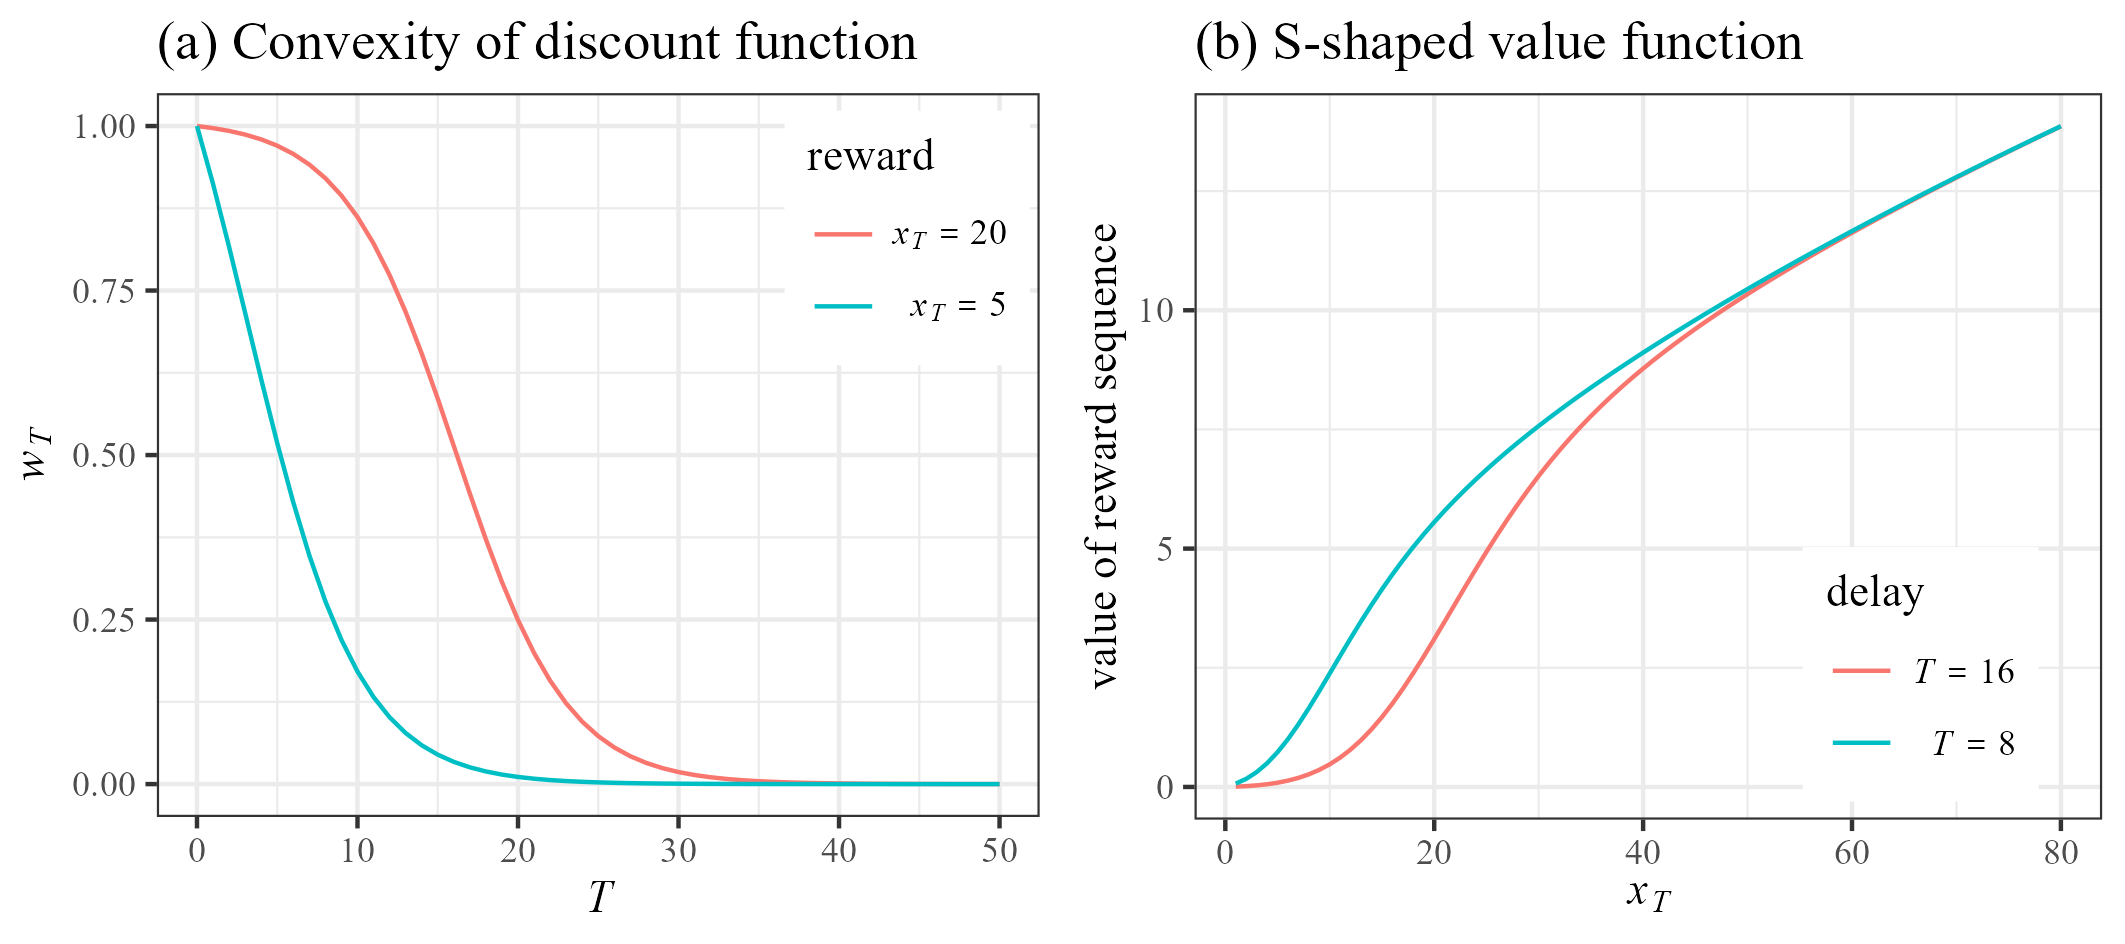
\includegraphics{images/plot-discount-value.png}
  \caption{Simulation results for choices between SS and LL. Value of reward sequence is calculated by $w_T\cdot u(x_T)$, where $w_T$ is calculated using Equation (2), $\delta=0.75$, $\lambda=1$, utility funtion $u(x)=x^{0.6}$.}
  \label{fig:plot-discount-value}
\end{figure}

\hypertarget{adus-offers-an-alternative-account-for-s-shaped-value-function}{%
\subsubsection{ADUS offers an alternative account for S-shaped value
function}\label{adus-offers-an-alternative-account-for-s-shaped-value-function}}

The S-shaped value function has been widely adopted by behavioral
economists. Some theories justifies it by reference-dependent utility
\citep{kahneman_prospect_1979, koszegi_model_2006}, while some others by
efficient coding of numerical values \citep{frydman_efficient_2021}. I
offer an account based on selective attention to sequential outcomes.

Imagine that a decision maker faces a choice between two lotteries. At
the moment when the choice is made, she does not receive any money from
either option. Thus, she may perceive the outcome of each option as
something that will happen in the future. She allocates attention
between the current period, which offers no reward, and the future
period when she could receive some money. When the amount of money that
she could receive is increased, not just does its utility increases, but
her attention is more directed towards that particular future period.

Assuming the decision maker perceives the outcome will be realized in
period \(T\), and in a certain state, the option she chooses yields
reward \(x_T\). We can use Equation (\ref{eq:w2}) to derive the value
function, i.e.~\(w_T\cdot u(x_T)\). Both utility function \(u(.)\) and
attention weight \(w_T\) exhibit diminishing sensitivity to the reward
outcome \(x_T\). However, when the reward is small enough, their product
may be convex . Notably, when the curvature of utility function
satisfies a certain condition, or the unit cost of information
\(\lambda\) is small enough, we can obverse a S-shaped value function.
Figure \ref{fig:plot-discount-value}(b) illustrates this.

\hypertarget{inattentive-decision-makers-perform-less-inconsistent-behaviors}{%
\subsubsection{Inattentive decision makers perform less inconsistent
behaviors}\label{inattentive-decision-makers-perform-less-inconsistent-behaviors}}

Imagine that a decision maker faces a task of allocating consumption
budget \(B\) across multiple periods, and in each period, she makes a
new consumption plan to optimize her attentional discounted utility.
Suppose she starts in period 0, then the task can be formulated as the
following optimization problem:

\[
\max_{c_0,...,c_T}\;\sum_{t=0}^T w_t\cdot u(c_t) \qquad s.t.\;\sum_{t=0}^T c_t=B  
\]

where \(c_t\) is consumption in period \(t\), \(w_t\) is the attention
weight, which is calculated with ADUS. I develop a numerical method to
solve this optimization problem.\footnote{The method combines the
  gradient projection method and F-W algorithm as a local optimizer, and
  use the basin-hopping method to achieve global optimization.}

Previously, researchers often employ ``present bias''
\citep{laibson_golden_1997} or ``naiveté'' \citep{odonoghue_doing_1999}
to account for the phenomenon of dynamic inconsistency in this context.
I provide an account based on attention weight updating.

I categorize each decision maker into two types based on how they
process information in this task - \emph{attentive} and
\emph{inattentive}. A decision maker is considered \emph{attentive} to
the decision task if, in each period, she remembers the information
about her consumption plan made in the last period and use it to update
attention weights. Otherwise, she is classified as \emph{inattentive}.

Suppose in period 0, the decision maker's initial attention weight is
proportional to \(\delta^t\), where \(0<\delta<1\). Given the decision
maker is impatient (\(\delta<1\)), she tends to consume more in earlier
periods within the planning horizon. Then in period 1, an
\emph{attentive} decision maker may update her initial attention weight
into \(w_t\) formed in period 0, which is proportional to
\(\delta^t\exp\{\frac{u(c_t)}{\lambda}\}\), and so on. Consequently, the
earlier periods, which originally has more planned consumption, will now
receive more (initial) attention weights than they did in the last
period. This leads to an increased preference for raising consumption
levels in such periods.

By contrast, if the decision maker is \emph{inattentive}, that is, she
does not mind much about the task and thus always forgets the
information about her prior consumption plans, then in period 1 and any
subsequent period, her initial attention weight will keep proportional
to \(\delta^t\). In this case, she could perform less inconsistent
behaviors than the attentive decision makers.
\ref{fig:plot-budget-dynamic} offers an illustration for the contrast.
The contrast may shed light on why some nudges that reduce the demand
for attention commitment, such as a default choice, can improve the
consistency in choices.

\begin{figure}
  \centering
  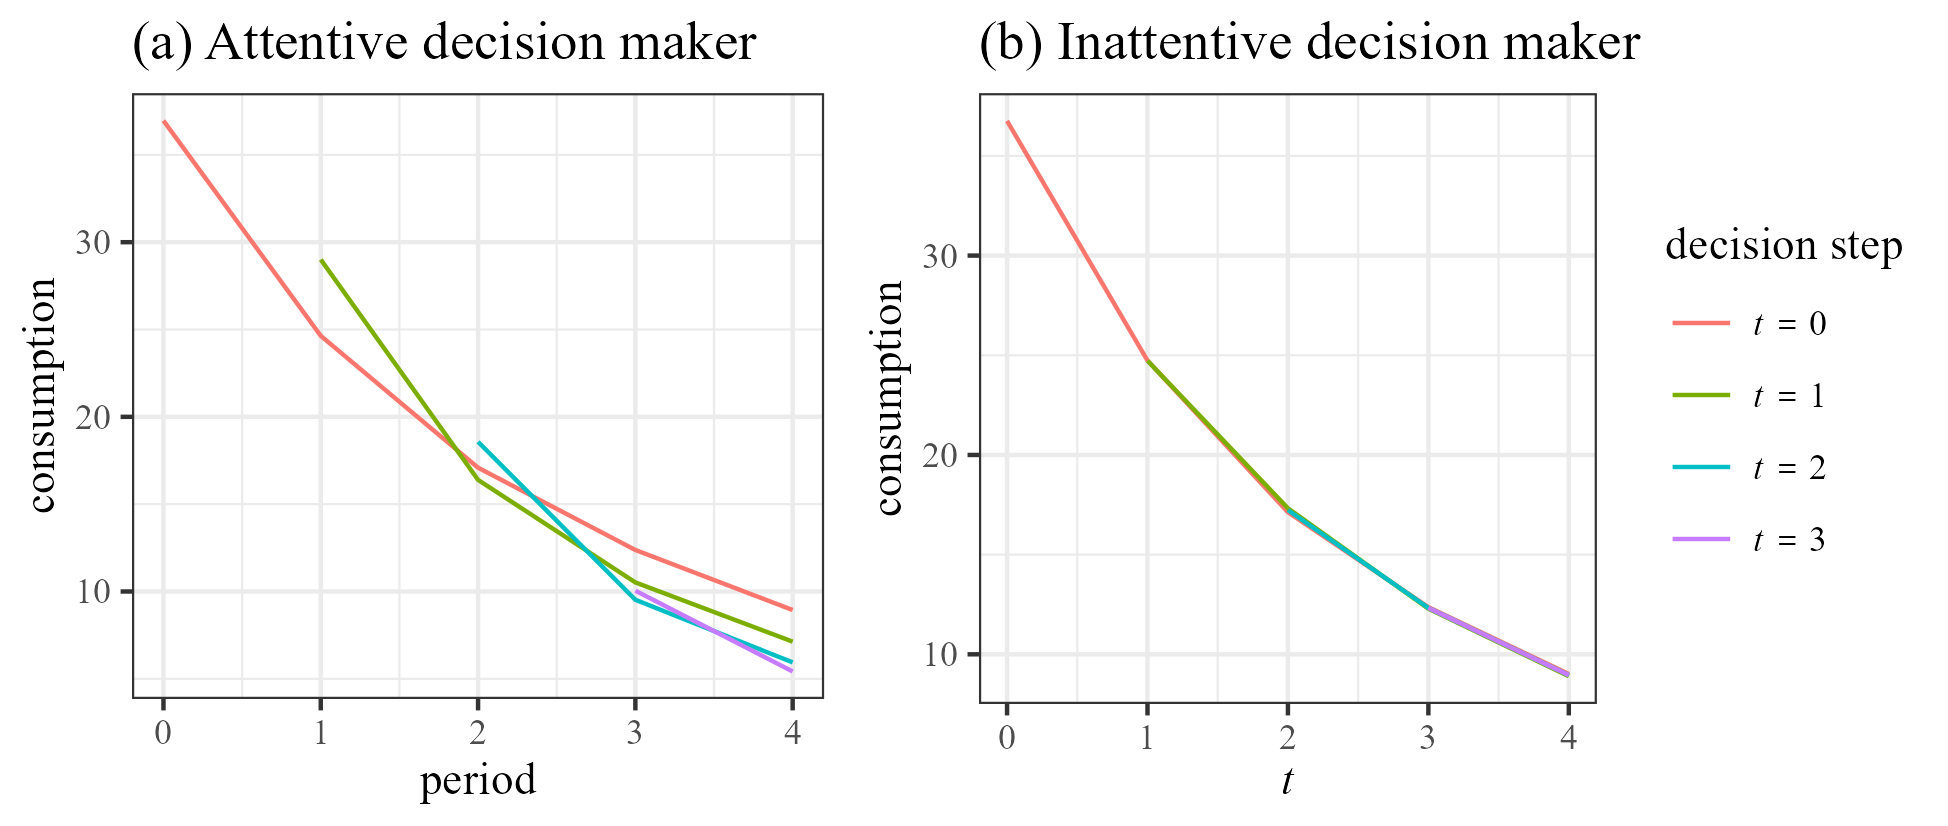
\includegraphics{images/plot-budget-dynamic.png}
  \caption{Simulation results for budget allocation. The decision maker allocations a budget of $B=100$ across five periods, $\delta=0.9$, $\lambda=70$. For each period $t$, utility funtion $u(x_t)=x_t^{0.6}$.}
  \label{fig:plot-budget-dynamic}
\end{figure}

\hypertarget{axiomization-of-adus}{%
\subsection{\texorpdfstring{Axiomization of ADUS
\label{axiom}}{Axiomization of ADUS }}\label{axiomization-of-adus}}

In this subsection, I provide an axiomatic rationale for using the
Shannon cost function in ADU. I firstly define the preference relation
\(\succsim\) that can be represented by ADU, then propose four axioms to
characterize the Shannon cost function.

\textbf{Definition 2}: Preference relation \(\succsim\) has an ADU
representation if and only if, for any stochastic reward sequence
\(X_T\), \(X'_{T'}\), we have \[
X_T \succsim X'_{T'} \Longleftrightarrow U(X_T)\geq U(X'_{T'})
\]where
\(U(X_T)=\sum_{S_T\in\mathcal{S}(X_T)}\sum_{t=0}^T w(s_t)u(s_t)\),
\(U(X'_{T'})=\sum_{S_{T'}\in\mathcal{S}(X'_{T'})}\sum_{t=0}^{T'}w'(s_t)u(s_t)\).
\(S_T\) and \(S'_{T'}\) are the potential realizations of sequence
\(X_T\) and \(X'_{T'}\), \(w(.)\) and \(w'(.)\) are the solutions to the
constrained optimal discounting problems for \(X_T\) and \(X'_{T'}\).

\textbf{Axiom 1}: (\emph{state independence}) For any reward sequence
\(X_T\), \(X'_T\), \(X''_T\) and \(\alpha\in(0,1)\), \(X_T\succ X'_T\)
implies
\(\alpha X_T+ (1-\alpha)X''_T \succ \alpha X'_T + (1-\alpha) X''_T\).

Axiom 1 implies that the determination of attention weights in one
potential realization of reward sequence will not interfere that in
another. If Axiom 1 is satisfied, each state in the constrained optimal
discounting problem has an independent solution.

\textbf{Axiom 2}: \emph{(sequential outcome betweenness)} For any
non-negative real number \(b\) and deterministic reward sequence
\(S_T\), let \(S_Tb\) denote \([s_0,s_1,...,s_T,b]\), there always
exists \(\alpha\in(0,1)\) such that \(S_Tb\sim \alpha S_T+(1-\alpha)b\).

Axiom 2 implies that if we add a new element to a given sequence, the
value of the new sequence will lies between the value of the original
sequence and the utility of the newly added element. The evidence of
``violation of dominance'' \citep{scholten_better_2014} may provide
support for this axiom.

\textbf{Axiom 3}: (\emph{sequential} \emph{bracket independence}) For
any non-negative real number \(b\), \(c\) and deterministic sequence
\(S_T\), if there exist \(\alpha_1\), \(\alpha_2\), \(\alpha_3\),
\(\beta_1\), \(\beta_2\in \mathbb{R}_{>0}\) such that
\[S_Tbc\sim \alpha_1S_T+\alpha_2b+\alpha_3c \quad\text{and}\quad S_Tbc\sim \beta_1S_T+\beta_2(bc)\]
where \(bc\) denotes a sequence with immediate reward \(b\) and period-1
reward \(c\), then we must have \(\alpha_1=\beta_1\).

Axiom 3 implies that if we segment a given sequence into different
elements, and find that the value of a linear combination of these
elements is equivalent to the value of the overall sequence, then in
this linear combination, the weight for any specific element can hold
constant no matter how we segment or bracket the other elements.

\textbf{Axiom 4}: (\emph{aggregate invariance of constant sequences})
For any deterministic sequences \(S_T\), \(S'_T\), given non-negative
real number \(c'\), \(c\) and \(\alpha\in(0,1)\), if
\(\alpha s'_t+(1-\alpha)c'\succ\alpha s_t+(1-\alpha)c\) holds for every
period \(t\), then
\(\alpha S'_T+(1-\alpha)c'\succ \alpha S_T+(1-\alpha)c\).

Axiom 4 implies that in a given sequence, if the utility of every
element plus an equal amount, then the overall utility of the sequence
should plus the same amount. Note in conventional discounted utility
models, sequences are typically assumed to be separable from each other.
In that case, any sequence can be \emph{aggregate invariant}. Thus,
Axiom 4 can be viewed as a weaker version of ``separability of
sequences''.

\textbf{Theorem 1}: \(\succsim\) has an ADUS representation if and only
if it has an ADU representation and satisfies Axiom 1-4.

\hypertarget{attention-allocation-over-sequential-outcomes-an-experimental-test}{%
\section{\texorpdfstring{Attention Allocation over Sequential Outcomes:
An Experimental Test
\label{3}}{Attention Allocation over Sequential Outcomes: An Experimental Test }}\label{attention-allocation-over-sequential-outcomes-an-experimental-test}}

\hypertarget{motivation}{%
\subsection{Motivation}\label{motivation}}

The second piece of work is an experimental test of the key assumptions
in my proposed model. Suppose a decision maker faces a choice between
receiving an immediate reward and receiving a sequence of rewards, and
when evaluating the sequence, she has only limited attention to allocate
across different time periods within the sequence. Then, if the length
of sequence is substantially extended, on average the attention that can
be allocated to each particular period would decrease. Under this
circumstance, any changes in the amount of rewards offered in each
period would have a smaller impact on her choice.

Moreover, suppose the decision maker tends to pay more attention to
periods with larger rewards. If the amount of reward offered in one
period is substantially increased, she would naturally shift more
attention to this particular period. Thus, the attention available to be
allocated to the rest of periods would decrease. Under this
circumstance, any changes in reward amounts for those other periods
would have a smaller impact on her choice.

\hypertarget{experimental-design}{%
\subsection{Experimental Design}\label{experimental-design}}

I designed a survey to test the above arguments. To illustrate how the
arguments will be tested, imagine that there are two options:

\setlength{\leftskip}{1cm}

A. ``receive £M today''

B. ``receive £X today and £Y in T months''

\setlength{\leftskip}{0pt}

Note option A is an immediate reward and option B is a sequence of
rewards. If people have to choose between option A and B, when either X
or Y increases (and the others are equal), more people should prefer
option B over A. Specifically, I make two predictions:

\textbf{Prediction 1}: If we increase T and keep Y unchanged, people
should be less sensitive to changes in X as the sequence length is
extended. In this case, increasing X by the same amount leads fewer
people to shift from option A to option B.

\textbf{Prediction 2}: If we increase Y but keep T unchanged, people
should also be less sensitive to changes in X as Y grabs a greater
amount of attention. In this case, increasing X by the same amount leads
fewer people to shift from option A to option B. The same is true for Y
when we increase X instead.

I plan to recruit N=150 participants via Prolific. In this survey,
participants need to answer 19 time preference questions and 1 risk
preference question. All participant are presented with the same
questions. Each time preference question consists of a list of choices.
In each row of the list, the participants are required to choose between
an immediate reward (the same as option A) and a sequence of rewards
(the same as option B). Figure \ref{fig:example-question} presents an
example question. The questions are designed with two conditions: in the
first condition, X increases by rows while the other variables (M, Y, T)
remain constant across the rows; in the second condition, it is Y that
increases by rows while the other variables remain constant within a
question. In the questions where X increases by rows, the value of X
goes up by 10 with each row, starting from 10 and going up to 90. The
same pattern is followed by Y as well.

\begin{figure}
  \centering
  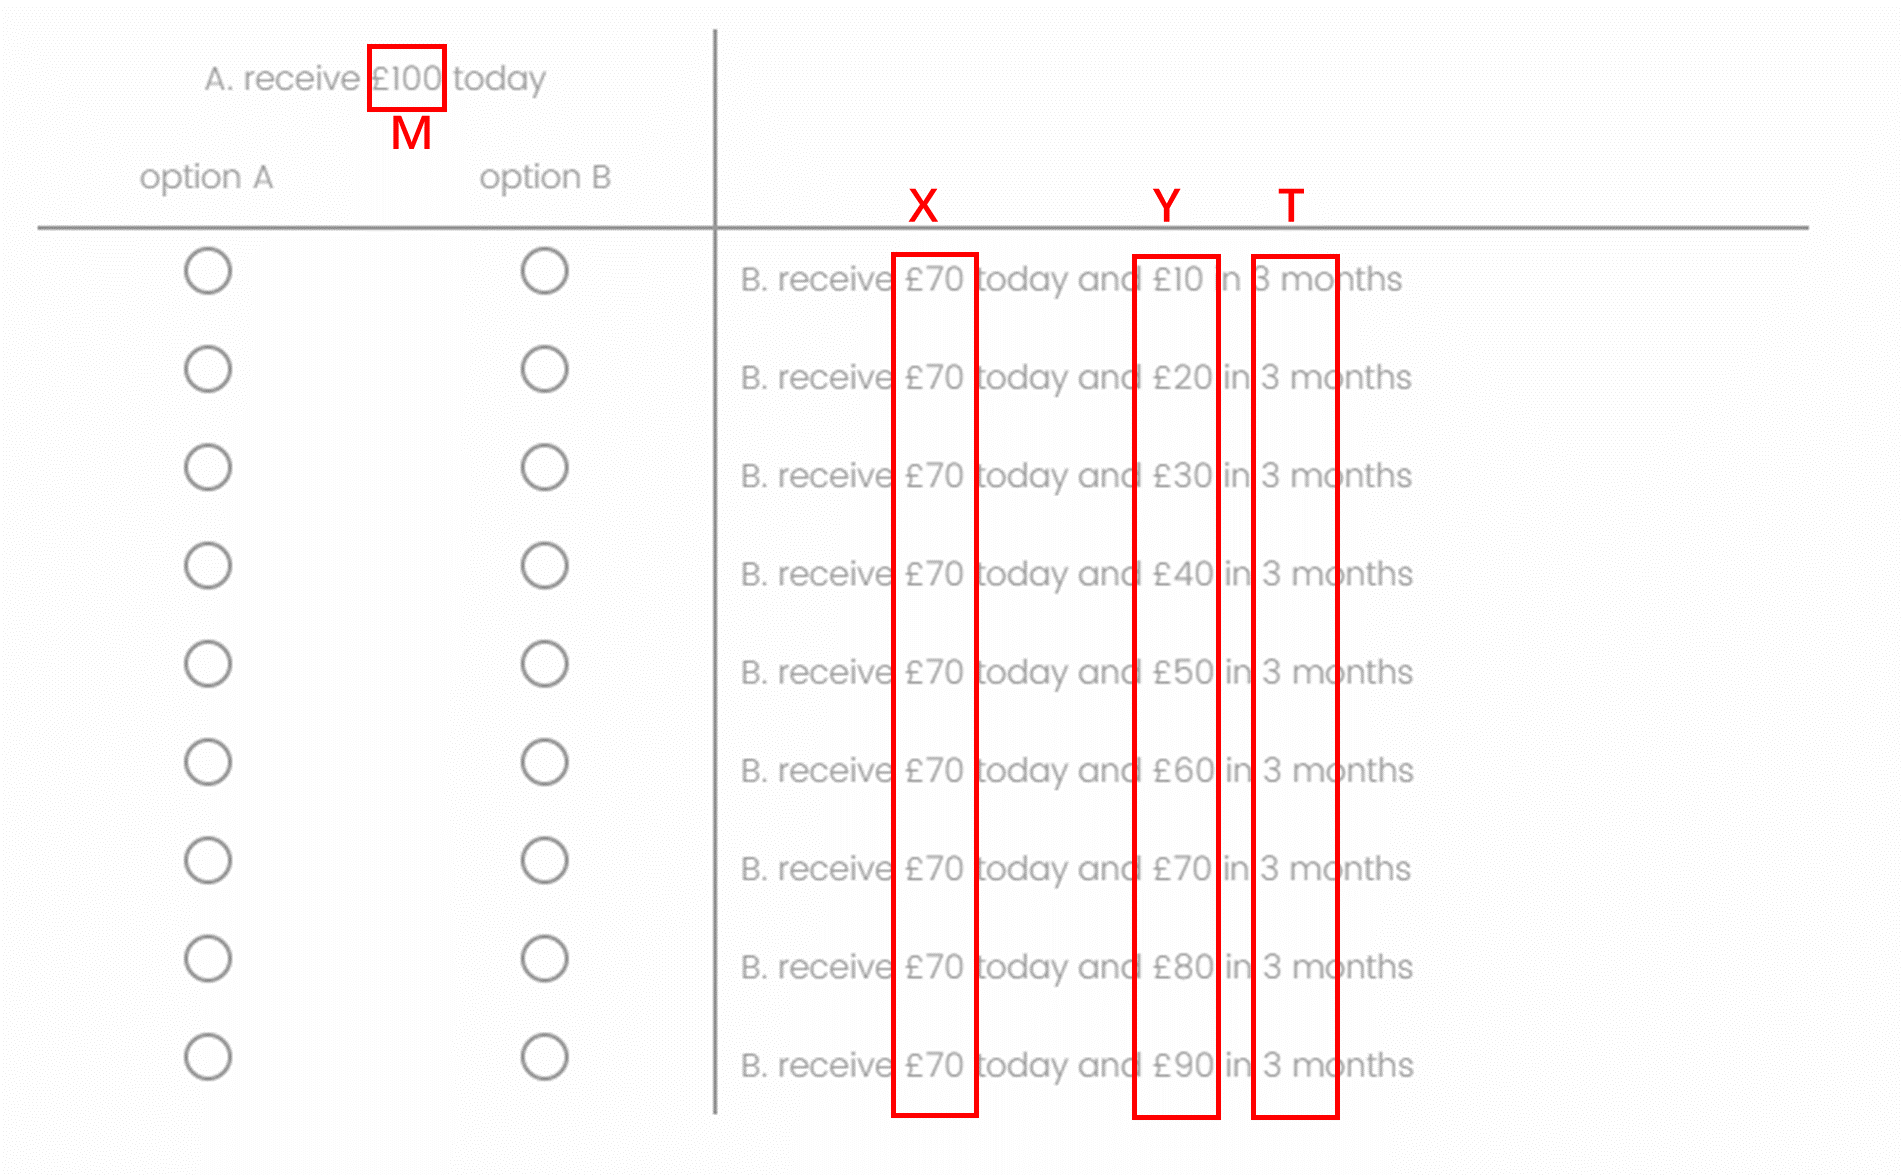
\includegraphics{images/example-question.png}
  \caption{Example question.}
  \label{fig:example-question}
\end{figure}

One of the time preference questions is set for attention check. For
attention check, M=50, X=100, T=3 and Y increases by rows. Given that
X\textgreater M, participants should consistently prefer option B to A
for every row in this question. For the rest of time preference
questions, M is selected from \{100,130\}, X and Y are selected from
\{50, 70, 90\}, T is selected from \{3, 9, 18\}. Table
\ref{tab:design-variable} shows how the values for M, X, Y and T are
distributed across these questions. All the questions are presented in a
random order.

At the end of the survey, there is a risk preference question. The risk
preference question is also a choice list. In each row of the list,
participants need to choose between a risky lottery (``win £100 with
probability 50\%'') and a sure amount of reward. The risky lottery is
constant across the rows while the sure reward increases by rows.
Measuring the risk preference will help us fit the utility function and
calibrate model parameters in statistical analysis.

\begin{longtable}{@{}ccc|ccc@{}}
\caption{Time preference questions}
\label{tab:design-variable}\\
\toprule
\multicolumn{3}{c}{X increases by rows} & \multicolumn{3}{c}{Y increases by rows} \\
\midrule
M (£) & X (£) & T (months) & M (£) & Y (£) & T (months) \\
\midrule
\endhead
\bottomrule
\endfoot
\endlastfoot
100 & 50 & 3 & 100 & 50 & 9 \\
100 & 70 & 3 & 100 & 70 & 9 \\
100 & 90 & 3 & 100 & 90 & 9 \\
100 & 70 & 9 & 130 & 50 & 9 \\
100 & 90 & 9 & 130 & 70 & 9 \\
100 & 90 & 18 & 130 & 90 & 9 \\
130 & 50 & 3 & \multicolumn{1}{c}{} & \multicolumn{1}{c}{} & \multicolumn{1}{c}{} \\
130 & 70 & 3 & \multicolumn{1}{c}{} & \multicolumn{1}{c}{} & \multicolumn{1}{c}{} \\
130 & 90 & 3 & \multicolumn{1}{c}{} & \multicolumn{1}{c}{} & \multicolumn{1}{c}{} \\
130 & 70 & 9 & \multicolumn{1}{c}{} & \multicolumn{1}{c}{} & \multicolumn{1}{c}{} \\
130 & 90 & 9 & \multicolumn{1}{c}{} & \multicolumn{1}{c}{} & \multicolumn{1}{c}{} \\
130 & 90 & 18 & \multicolumn{1}{c}{} & \multicolumn{1}{c}{} & \multicolumn{1}{c}{} \\
\bottomrule
\end{longtable}

For statistical analysis, the key dependent variable will be the choice
between option A and B in each row of time preference questions. I will
run logistic regressions for two conditions respectively. In the
condition that X increases by rows, the main independent variables will
be M, X, and the interaction effects among Y, T and X. To validate
Prediction 1, I will test whether for participants the likelihood of
choosing B is significantly less sensitive to X while T being larger. To
validate Prediction 2, I will test whether the likelihood of choosing B
is significantly less sensitive to X while Y being larger. The condition
that Y increases by rows is only used for validating Prediction 2. The
main independent variables will be M, Y, and the interaction effects
among X, T and Y. I will test whether the likelihood of choosing B is
significantly less sensitive to Y while X being larger. For an
additional analysis, I will fit multiple models to data. These models
include exponential, hyperbolic, and quasi-hyperbolic discounting, and a
variant of attentional discounted utility. The purpose of this
additional analysis is to explore whether putting a non-linear structure
that captures the key properties of attention in the discounted utility
framework can improve predictive performance.

\begin{figure}
  \centering
  \resizebox{0.6\textwidth}{!}{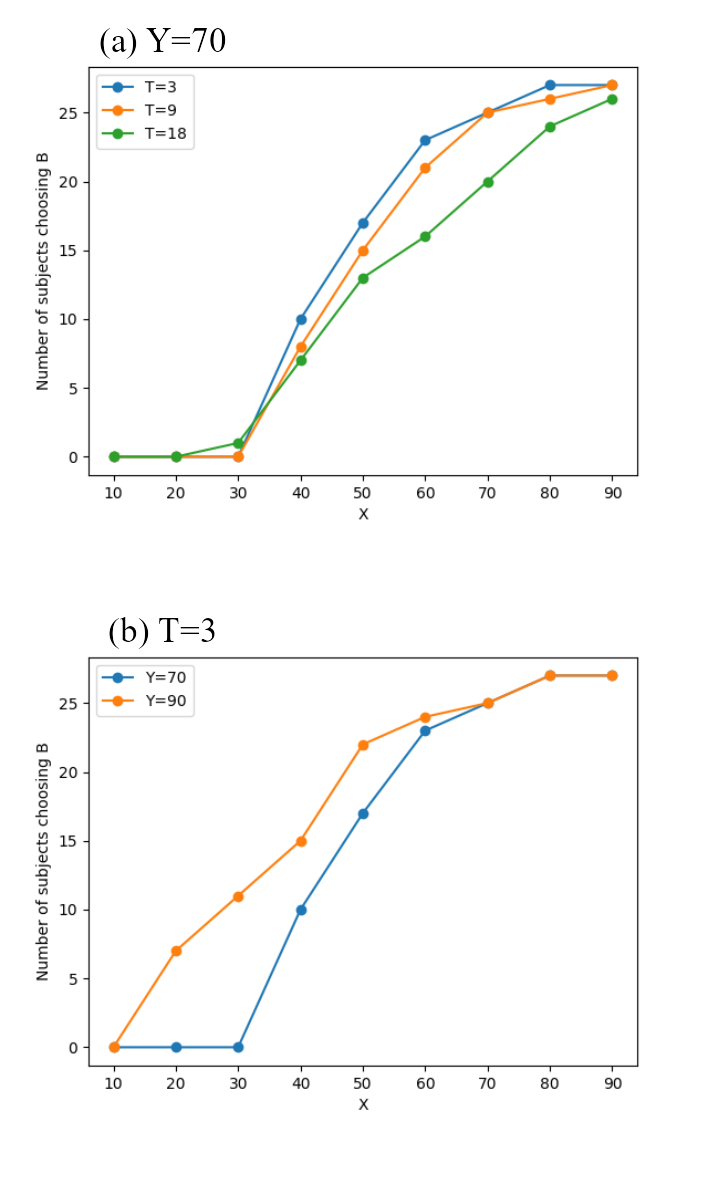
\includegraphics{images/pilot-result.png}}
  \caption{Behavioral patterns observed in a pilot study. X increases by rows, M=100.}
  \label{fig:pilot-result}
\end{figure}

\hypertarget{pilot-study}{%
\subsection{Pilot Study}\label{pilot-study}}

I did two pilot studies in the last month. Each pilot study contains
N=30 participants. Given the sample size is small, I do not perform a
formal analysis here. However, some behavioral patterns observed in
pilot studies can help illustrate how my predictions may be validated.
See Figure \ref{fig:pilot-result} for details.

It can be observed that people are more likely to choose option B when X
grows larger. However, the rate at which this likelihood of choosing B
grows varies across settings. In Figure \ref{fig:pilot-result}(a), the
blue curve (T=3) has is the sharpest and the green curve (T=18) is the
flattest. Thus, people may be less sensitive to the changes in X when
T=18 than when T=3, which is in line with Prediction 1. In Figure
\ref{fig:pilot-result}(b), the blue curve (Y=70) is sharper than the
orange curve (Y=90). Thus, people may be less sensitive to the changes
in X when Y=90 than when Y=70, which is in line with Prediction 2.

\hypertarget{valuation-of-risk-and-effort}{%
\section{\texorpdfstring{Valuation of Risk and Effort
\label{4}}{Valuation of Risk and Effort }}\label{valuation-of-risk-and-effort}}

\hypertarget{experimental-procedure}{%
\subsection{Experimental Procedure}\label{experimental-procedure}}

The third piece of work (in design) aims to test how people jointly
valuate risk and effort in an experiment. The experiment consists of
multiple rounds of effort-exertion decision tasks. In each round, there
are two types of balls on the screen -- red balls and blue balls.
Participants can change the color of each ball by clicking on it and
completing a simple real-effort task (entering a CAPTCHA). If the
original color is blue, then it will be changed to red, and vice versa.
There is no limit on the times of color change. After they make such
changes, the participants can click a button then a ball will be
randomly drawn from all the balls presented on the screen. The
participants can get different levels of reward when different colors of
balls are drawn. Suppose the reward for a blue ball is greater than that
for a red ball, in each round, the participants will be more inclined to
change red balls to blue balls, by making efforts. They need to balance
the benefit of increasing the probability of drawing a high-value ball,
and the cost of making efforts to change the colors. Figure
\ref{fig:demo} presents a screenshot of this task.

\begin{figure}[h]
  \centering
  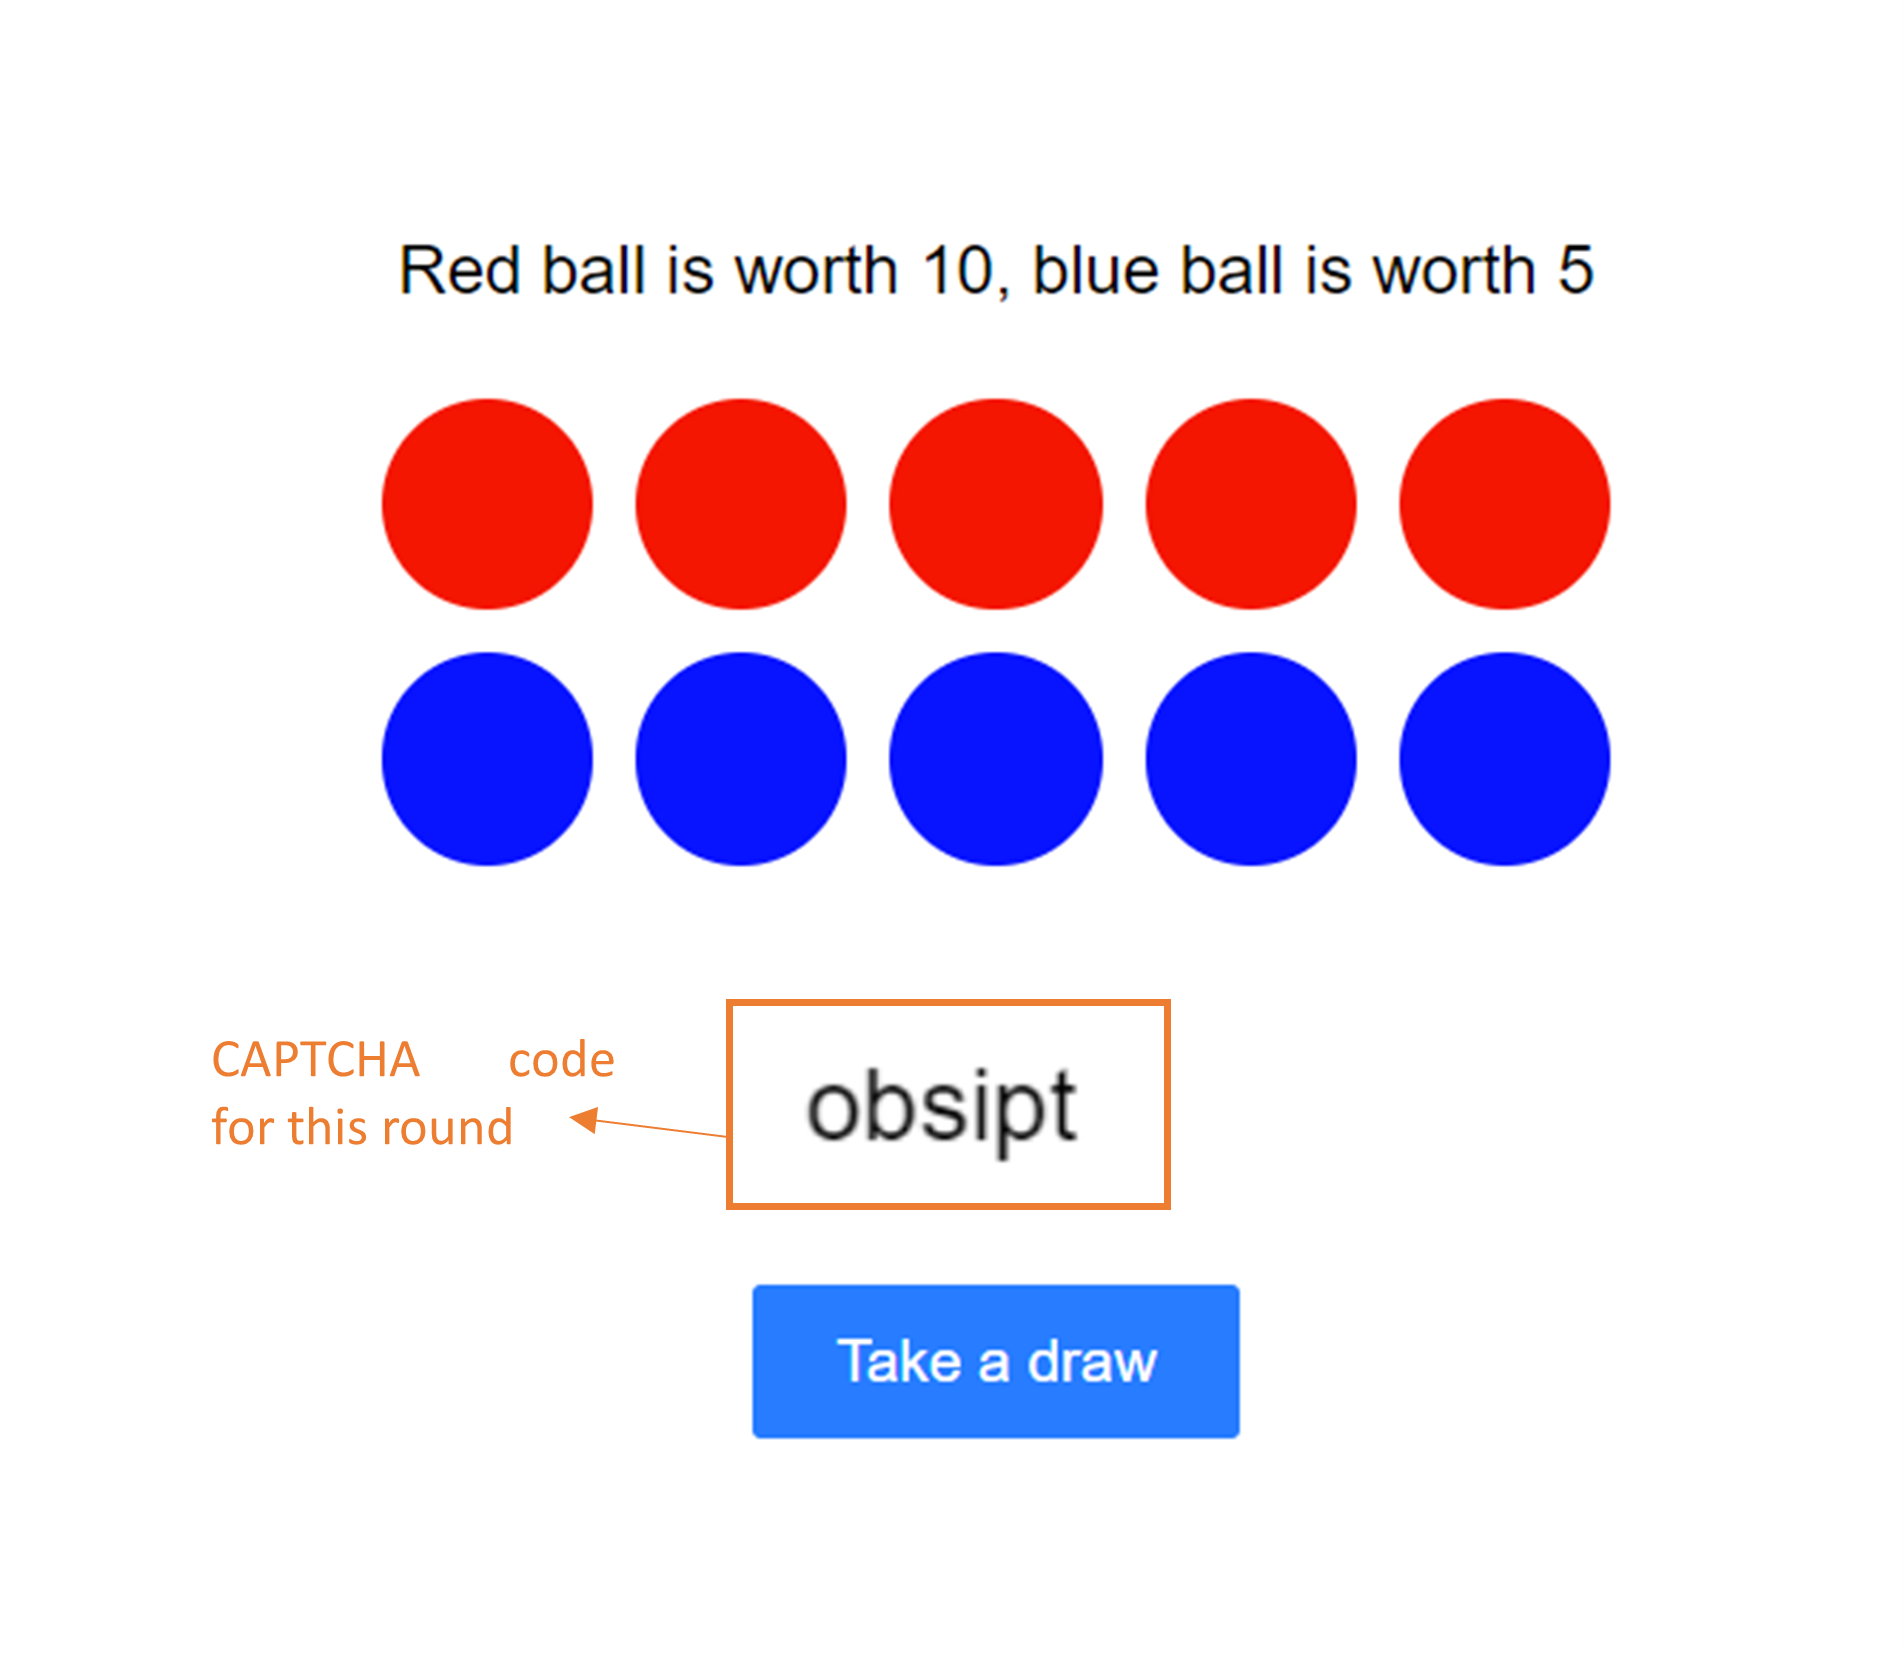
\includegraphics[width=0.75\textwidth]{images/screenshot-demo.png}
  \caption{A screenshot of the experimental program (demo). After clicking on any of the balls, a pop-up window will appear and ask people to enter the CAPTCHA code, in order to change its color. The program is written in Javascript.}
  \label{fig:demo}
\end{figure}

\hypertarget{behavioral-implications-1}{%
\subsection{Behavioral Implications}\label{behavioral-implications-1}}

This experimental approach can help us examine how the cost of effort
may impact decision making. While researchers today understand a lot
about risk preferences, there is still limited evidence on the
willingness to exert effort. By this approach, we can use our knowledge
about risk preferences to elicit the preferences of effort exertion, and
to characterize the effort cost function.

Moreover, although there has been some theories considering effort as a
necessary input for decision making, the effort discussed in such
theories, e.g.~attention, is usually at the cognitive level; whereas,
this experiment also involves physical effort or the effort to actually
implement the decision. The setting in this experiment is consistent
with that set up in such theories, therefore it allows a direct
comparison between the two forms of effort. For example, in rational
inattention theories \citep{matejka_rational_2015}, it is typically
assumed that people should make a choice between different items and it
costs some (cognitive) effort to acquire the value information of each
item. When less effort is exerted, people may perform a higher degree of
randomness in those choices (just like the red and blue balls have a
nearly even chance to be drawn). Such a kind of comparisons may lead to
a new theory of effort cost in future research.

This experiment also has a real-world implication. In experiment,
participants are required to exert greater effort to increase their
chances of drawing a high-value ball. In reality, when we work harder,
it is often that we are more likely to achieve a good outcome. For
instance, we may work hard on a paper to increase the probability that
it is published on a top journal, or on researching and adjusting
investment portfolio in order to get a higher return in financial
markets. Thus, what we learn from the experiment may also shed light on
these research fields.

\hypertarget{time-schedule}{%
\section{Time Schedule}\label{time-schedule}}

\begin{longtable}{@{}p{0.3\linewidth}p{0.6\linewidth}@{}}
\caption{Timeline}
\label{tab:timeline}\\
\toprule
Time & Progress \\* \midrule
\endhead
%
Aug, 2023 & \begin{tabular}[t]{@{}p{\linewidth}@{}}
1. Refine empirical analysis on the behavioral implications of ADU (Project 1)\\     2. Implement the experiment about the role of attention in intertemporal choice (Project 2)\\
\\
\end{tabular} \\* 
Sept, 2023 & \begin{tabular}[t]{@{}p{\linewidth}@{}}
1. Complete the relevant proofs (Project 1)\\     
2. Analyze the experimental results and design a follow-up test (Project 2)\\
\\
\end{tabular} \\* 
Oct, 2023 & \begin{tabular}[t]{@{}p{\linewidth}@{}}
1. Finish the first draft of the paper (Project 1)\\  
2. Complete the required procedures for a follow-up test (Project 2)\\ 
3. Complete the experimental design (Project 3)\\
\\
\end{tabular} \\* 
Nov, 2023 & \begin{tabular}[t]{@{}p{\linewidth}@{}}
1. Collect data from the follow-up test and conduct relevant statistical analyses  (Project 2)\\ 
2. Complete the required procedures for running the experiment (Project 3)\\
\\
\end{tabular} \\* 
Dec, 2023 & Implement the experiment about valuation of risk and effort (Project 3) \\
\\* 
Jan-March, 2024 & Draft research papers and consider additional analyses (Project 2\&3) \\ 
\\* 
Apr-July, 2024 & Complete the thesis 
\\* \bottomrule
\end{longtable}

\renewcommand\refname{Reference}
  \bibliography{reference.bib}

\end{document}
